%\documentclass[tikz, border=5pt]{standalone}
\begin{document}
	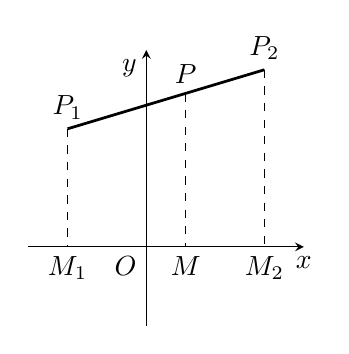
\begin{tikzpicture}[>=stealth, scale=0.5] % 箭头样式为stealth,
		
		% 绘制坐标轴
		\draw[->] (-3,0) -- (4,0) node[below] {$x$};      % x轴(带箭头和标签)
		\draw[->] (0,-2) -- (0,5) node[below left] {$y$}; % y轴(带箭头和标签)
		\node at (0,0) [below left] {$O$};                % 原点O的标签
		
		% 定义各关键点坐标
		\coordinate (P1) at (-2,3); % 点P₁
		\coordinate (P2) at (3,4.5);  % 点P₂
		\coordinate (P) at (1,3.9);  % 点P
		\coordinate (M1) at (-2,0); % 点M₁
		\coordinate (M2) at (3,0);  % 点M₂
		\coordinate (M) at (1,0);   % 点M
		
		% 绘制连接P₁和P₂的直线
		\draw[line width=1pt] (P1) -- (P2);
		
		% 绘制虚线辅助线(矩形的边)
		\draw[dashed] (P1) -- (M1); % P₁到x轴的虚线
		\draw[dashed] (P2) -- (M2); % P₂到x轴的虚线
		\draw[dashed] (P) -- (M);  % M到P的虚线
		
		% 标记各点的标签
		\node at (P1) [above] {$P_1$};
		\node at (P2) [above]  {$P_2$};
		\node at (P) [above]  {$P$};
		\node at (M1) [below]  {$M_1$};
		\node at (M2) [below]  {$M_2$};
		\node at (M) [below]  {$M$};
		
	\end{tikzpicture}
\end{document}
